\documentclass[11pt]{beamer}
\usepackage{pgf-umlsd}
\usepackage{tikz}
\usepackage{tabularx}
\usepackage[center]{caption}
\usepackage{makecell}
\usepackage{multirow}
\usepackage{listings}
\usepackage{listings} 

\definecolor{verylightgray}{rgb}{.8,.8,.8}
\definecolor{lightblue}{rgb}{190,218,255}
\definecolor{orangeyellow}{rgb}{253,201,0}
\definecolor{lightpink}{rgb}{255,243,254}

\definecolor{myorange}{HTML}{FDC900}
\definecolor{myblue}{HTML}{BAD4FF}
\definecolor{mypink}{HTML}{F3D2FE}
\definecolor{mygray}{HTML}{4A4A4A}

\lstdefinelanguage{modelLang}{
% 	commentstyle=\color{gray}\ttfamily,
    commentstyle=\color{green}, % style of comments
    morecomment=[l][\color{green!40!black}\itshape]{//},
	morecomment=[s][\color{green!40!black}\itshape]{/*}{*/},
	stringstyle=\color{red}\ttfamily,
	morestring=[b]',
	morestring=[b]",
	keywordstyle=[2]\color{teal}\bfseries,
	keywords=[3]{participant, identified, by, asset, default, optional, transaction, rule, description, operation, resource, condition, action},	% environment variables
	keywordstyle=[3]\color{violet}\bfseries,
	identifierstyle=\color{black},
	sensitive=true,
	keywords=[1]{Address, Status, Data, DataPublisher, PublishData, metaData, info, ModifyData, VerifyData, PublishTransaction}, % generic keywords including crypto operations
	keywordstyle=[1]\color{blue}\bfseries,
	keywords=[2]{ String, DateTime, Double, Integer}	% types; money and time units
}

\lstset{
	language=modelLang,
	backgroundcolor=\color{verylightgray!30},
	extendedchars=true,
	basicstyle=\linespread{1}\scriptsize\ttfamily,
	showstringspaces=false,
	showspaces=false,
	numbers=none,
% 	numberstyle=\tiny\sffamily,
% 	numbersep=5pt,
	tabsize=2,
	breaklines=true,
	showtabs=false,
	captionpos=b,
	numberbychapter=false
}

% \lstdefinestyle{numbers}
% {numbers=left, stepnumber=1, numberstyle=\tiny, numbersep=10pt}
% \lstdefinestyle{nonumbers}
% {numbers=none}
%%%%%%%% tema e cor %%%%%%%%
\mode<presentation> {
\usetheme{Madrid}
%\usecolortheme{albatross}
}


\usepackage[utf8]{inputenc}
\usepackage{graphicx} 
\usepackage{booktabs} 



\institute[HCMUT] 
{
%================= logos no meio =====================
\vspace*{-0.35cm}

\includegraphics[width=1.8cm]{img/Logo-hcmut.png}
\vspace*{0.35cm}\\
Ho Chi Minh University of Technology  -- HCMUT \\
%\medskip
%\texttt{\{lods.eng,ronety\}@uea.edu.br} % emails
}
\date{\today}

\AtBeginSection[]
{
\begin{frame}
\frametitle{Contents}
\tableofcontents[currentsection]
\end{frame}
}

%%%%%%%% titulo e subtitulo %%%%%%%%
\title[Blockchain-based Open Data]{Blockchain-based Open Data: An Approach for Resolving Data Integrity and Transparency} 

%%%%%%%% nome dos autores %%%%%%%%
\author[Dinh-Duc Truong]
{Dinh-Duc~Truong}
% Van-Thanh~Nguyen, Quoc-Bao~Nguyen, Huynh-Huy~Nguyen, Tuan-Anh~Tran,  Nhat-Quang~Le, An-Khuong~Nguyen} 

\begin{document}
\begin{frame}
\titlepage 

\end{frame}

\begin{frame}
\frametitle{Contents} 
\tableofcontents 
\end{frame}

%%%%%%%% slides %%%%%%%%
\section{Introduction} 
\begin{frame}{Introduction}{Motivation}
    \begin{itemize}
        \setbeamercovered{transparent}
        %\onslide<1->{\item The term \textit{open data} nowadays is popularized and becomes trending in many cities or nations around the world.}
        \onslide<1->{\item Building a smart city or electronic government trend.
              % requires a huge amount of data sets.
              }
              % Sharing data between a federal or citizens is an efficient method that can save time and effort for data preparation
              \onslide<2->{\item The security aspects of \textit{open data} -- CIA triangle.}
    \end{itemize}
    \uncover<3->{
        \begin{figure}
            \centering
            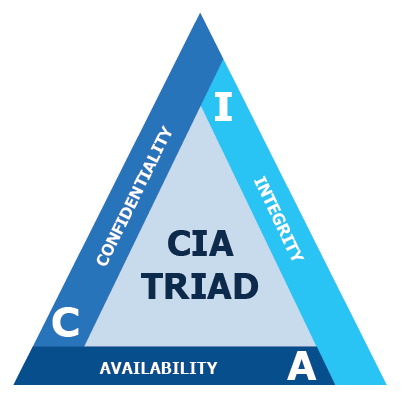
\includegraphics[width=.3\textwidth,height=.3\textwidth]{img/CIA-Triangle-02.png}
            % \caption{Open data}
            %   \label{fig:arOv}
        \end{figure}
    }
    \begin{itemize}
        \setbeamercovered{transparent}
        \onslide<3->{
        %   \item Attacking on websites or databases have been going on and inflict tremendous damage because of centralize system disadvantage.\\
        \onslide<4->{\item Centralize system disadvantage \\
              \uncover<5->{$=>$ Invalid data sets led people to make bad decisions.}
              }
              }
    \end{itemize}
\end{frame}
\begin{frame}{Introduction}{Motivation}
    Here are a few famous attacks since 2008\footnote{https://www.itsecurityguru.org/2016/11/29/2017-year-data-integrity-breach/}:
    \begin{itemize}
        \item 2008 - Hackers infiltrate the Brazilian governments systems and inflate the logging quotas to disrupt logging industry.
        \item 2010 - Hackers use the Stuxnet Worm to make minor changes in Iran’s nuclear power program in an attempt to destroy it.
        \item 2015 - Anonymous begin releasing financial reports exposing firms in the US and China trying to cheat the stock market.
              % In one case, damaging the brand reputation of REXLot Holdings, a games developer, which had inflated its revenues
        \item 2015 - JP Morgan Chase was breached with subsequent attempts at market manipulation.
        \item 2016 - Both the World Anti-Doping Agency and Democratic National Committee are breached with hackers manipulating their data to embarrass the organisations.
    \end{itemize}
\end{frame}

% \begin{frame}{Introduction}{Solution}
%     \setbeamercovered{transparent}
%     \begin{itemize}

%         % \item<2-> Blockchain and open data: a match made in heaven?
%         \onslide<1->{\item \textbf{Our idea}: Blockchain + IPFS +  Open data.}
%     \end{itemize}
%     \begin{figure}
%         \centering
%         \includegraphics<2->[width=.6\textwidth,height=.25\textwidth]{img/intro.png}
%         % \caption{Open data}
%         % \label{fig:arOv}
%     \end{figure}
% \end{frame}


\section{Background}
\begin{frame}{Open data}{Definition}
    \begin{block}{Open data}
        \textit{``Open data is data that can be freely used, re-used and redistributed by anyone - subject only, at most, to the requirement to attribute and share alike''}.
    \end{block}
    \pause
    \begin{figure}
        \centering
        
\includegraphics[width=.6\textwidth,height=.4\textwidth]{img/OSM.png}
        % \caption{Open data}
        % \label{fig:arOv}
    \end{figure}
\end{frame}

\begin{frame}{Open data}{Properties}
    \begin{itemize}
        \setbeamercovered{transparent}
        \onslide<1->{\item[+] Technically open:
              \begin{itemize}
                  \uncover<2-> {
                  %   \item The citizens access to all unrestricted data sets easily.
                  \item Accessing to data sets: unrestricted, easy.
                        }
                        \uncover<3-> {
                        % \item Data sets are available for downloading in multiple formats readable by computers.
                  \item Data formats: computer-readable.
                        }
                        % \uncover<4-> {\item The Open API provides the citizens with access to the data sets.}
              \end{itemize}}
              \pause
              \pause
              \pause
              %   \pause
              \onslide<4->{\item[+] Legally open:
              \begin{itemize}
                  \uncover<5-> {\item No restrictions on use and/or redistribution.}
                        % For example, citizens can use the data sets for either commercial or non-commercial purposes
                        % \uncover<6-> {\item Data sets are available under an open license.}
              \end{itemize}}
    \end{itemize}
    \uncover<6->{
        \begin{figure}
            \centering
            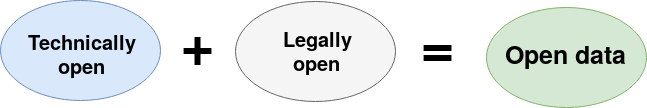
\includegraphics[width=.8\textwidth,height=.2\textwidth]{img/techleg.png}
            % \caption{Open data}
            % \label{fig:arOv}
        \end{figure}
    }
\end{frame}

\begin{frame}{Open data}{Benefits}
    % The \textit{Open data} is expected to bring a lot of benefits to:
    \vspace{0.3cm}
    \begin{columns}
        \setbeamercovered{transparent}
        \onslide<1->{
            \begin{column}{0.5\textwidth}
                +The government:
                \begin{itemize}
                    \uncover<2->{\item Improving transparency and publicity.}
                          \uncover<3->{\item Reducing the government operation cost.}
                \end{itemize}
            \end{column}}
        % \only<1-3>{
        %     \begin{column}{0.5\textwidth}
        %     \end{column}}
        \pause
        \pause
        \pause
        \onslide<4->{
            \begin{column}{0.5\textwidth}
                +The citizens:
                \begin{itemize}
                    \uncover<5->{\item Monitoring the government operation.}
                          \uncover<6->{\item Accessing to larger data resources.}
                \end{itemize}
            \end{column}}
    \end{columns}
    \uncover<7->{
        \begin{figure}
            \centering
            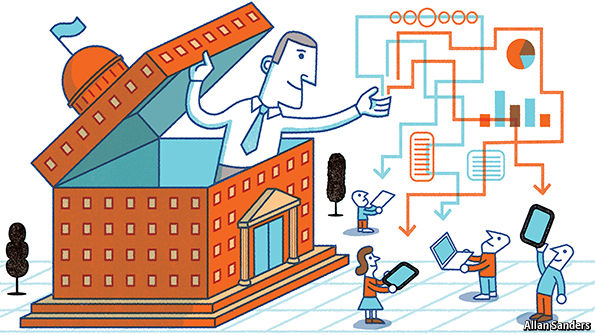
\includegraphics[width=.6\textwidth,height=.25\textwidth]{img/opendata.jpg}
            % \caption{Open data}
            % \label{fig:arOv}
        \end{figure}}
\end{frame}

\begin{frame}{Open data}{Security issues}
    % \begin{block}{Security analysis of open data}
    \setbeamercovered{transparent}
    \begin{itemize}
        \onslide<1->{\item In terms of the law:
              % it must be ensured that there is no legal violation, no disclosure of economic secrets, personal information and especially information on infrastructure.
              \begin{itemize}
                  \item<2-> no legal violation;
                  \item<3-> no disclosure of economic secrets;
                  \item<4-> no leak of personal information;
                  \item<5-> no publication of information on infrastructure.
              \end{itemize}
              }
              \pause
              \pause
              \pause
              \pause
              \pause
              \onslide<6->{\item  In terms of the technical:
              %    open data systems need to ensure  the  availability  and  integrity  of  data.
              \begin{itemize}
                  \item<7-> ensuring the availability and integrity of data.
              \end{itemize}
              }
    \end{itemize}
    % \end{block}
\end{frame}

\begin{frame}{Blockchain}{Definition}
    \begin{block}{Blockchain}
        % A \textbf{blockchain} is an electronic ledger that stores encrypted, authenticated and shared events in the format of \textit{transactions} in a decentralized network
        %  using consensus protocols.
        A \textbf{blockchain} is a growing list of records, called blocks, that are linked using cryptography. Each block contains a cryptographic
        hash of the previous block, a timestamp, and transaction data.
    \end{block}
    % \vspace{0.5cm}
    \begin{columns}
        \onslide<2->{
            \begin{column}{0.6\textwidth}
                \begin{figure}
                    \centering
                    \includegraphics<2->[width=0.9\textwidth,height=.4\textwidth]{img/blockchain.png}
                    % \caption{Blockchain}
                    % \label{fig:arOv}
                \end{figure}
            \end{column}
        }
        \onslide<3->{
            \begin{column}{0.4\textwidth}
                Types of blockchain:
                \begin{itemize}
                    \item<4-> Public blockchain.
                    \item<5-> Private blockchain.
                    \item<6-> Consortium blockchain.
                \end{itemize}
            \end{column}
        }
    \end{columns}
\end{frame}
\begin{frame}{Hyperledger Fabric}{Definition}
    % \begin{block}{
    Hyperledger Fabric:
    % }
    \begin{itemize}
        \setbeamercovered{transparent}
        \uncover<2->{
        % \item Hyperledger Fabric is a \textbf{private blockchain} developed and maintained by Linux Foundation and IBM Corporation.
        \item Private blockchain.
              }
              \uncover<3->{
              %   \item Hyperledger Fabric provides a flexible way to configure consensus protocol as well as customize transactions to fit with specific goals.
        \item Flexible consensus protocol.
              }
    \end{itemize}
    % \end{block}
    \uncover<4->{
        \begin{figure}
            \centering
            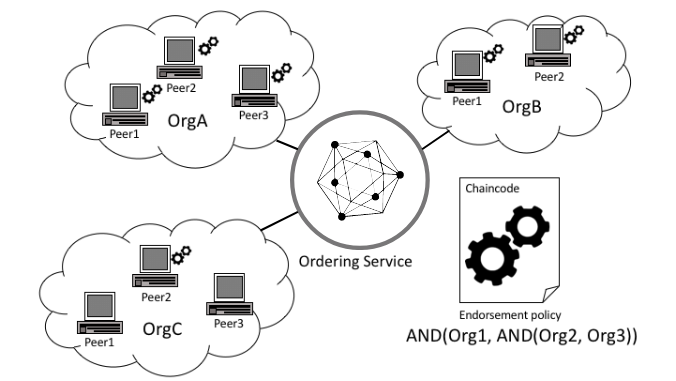
\includegraphics[width=.7\textwidth,height=.35\textwidth]{img/HF.png}
            % \caption{Hyperledger Fabric}
            % \label{fig:arOv}
        \end{figure}}
\end{frame}

\begin{frame}{InterPlanetary File System}{Definition}
    \begin{block}{IPFS}
        InterPlanetary File System, IPFS for short, is a peer-to-peer distributed file system for storing and sharing hypermedia files over a network.
    \end{block}
    \pause
    \begin{figure}
        \centering
        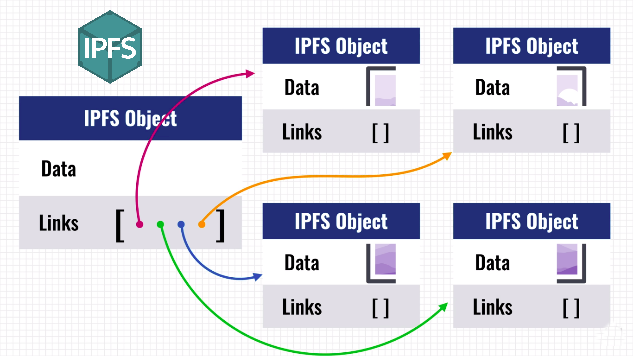
\includegraphics[width=.7\textwidth,height=.35\textwidth]{img/IPFS.png}
        % \caption{InterPlanetary File System}
        % \label{fig:arOv}
    \end{figure}
\end{frame}


\section{Related works}
\begin{frame}{Related works}{Non blockchain-based}
    \setbeamercovered{transparent}
    \begin{itemize}
        \onslide<1->{\item[1.]US open data portal
              \begin{itemize}
                  \uncover<2->{\item since 2009;}
                        \uncover<3->{\item provides a number of 229,371 data sets in various formats and related to many fields.}
                        %  such as agriculture, ecosystems, education, energy, finance, health, natural disasters, science, and research.}
              \end{itemize}
              }
              \pause
              \pause
              \pause
              \onslide<4->{\item[2.]Ho Chi Minh open data portal
              \begin{itemize}
                  \uncover<5->{\item since 2017;}
                        %   The portal is expected to have integration with some important databases including medical, education, invest, environment, etc.}
                        \uncover<6->{\item still thin in the content due to lacking data sets.}
              \end{itemize}
              }
    \end{itemize}
\end{frame}
\begin{frame}{Related works}{Blockchain-based}
    \begin{itemize}
        \item[3.]Vienna open data portal
              \setbeamercovered{transparent}
              \begin{itemize}
                  \uncover<2->{\item called "Data Notarization Blockchain" in 2018;}
                        %   Austria government has applied the blockchain technology to the open data portal of Vienna and successfully demonstrated under a project named ``Data Notarization Blockchain'' in 2018.}
                        \uncover<3->{\item uses public blockchain.}
                        % Once a contributor publishes a data set, a checksum of it will be stored on the public blockchain network for validating the content of the data.}
              \end{itemize}

    \end{itemize}
    \uncover<4->{
        \begin{figure}
            \centering
            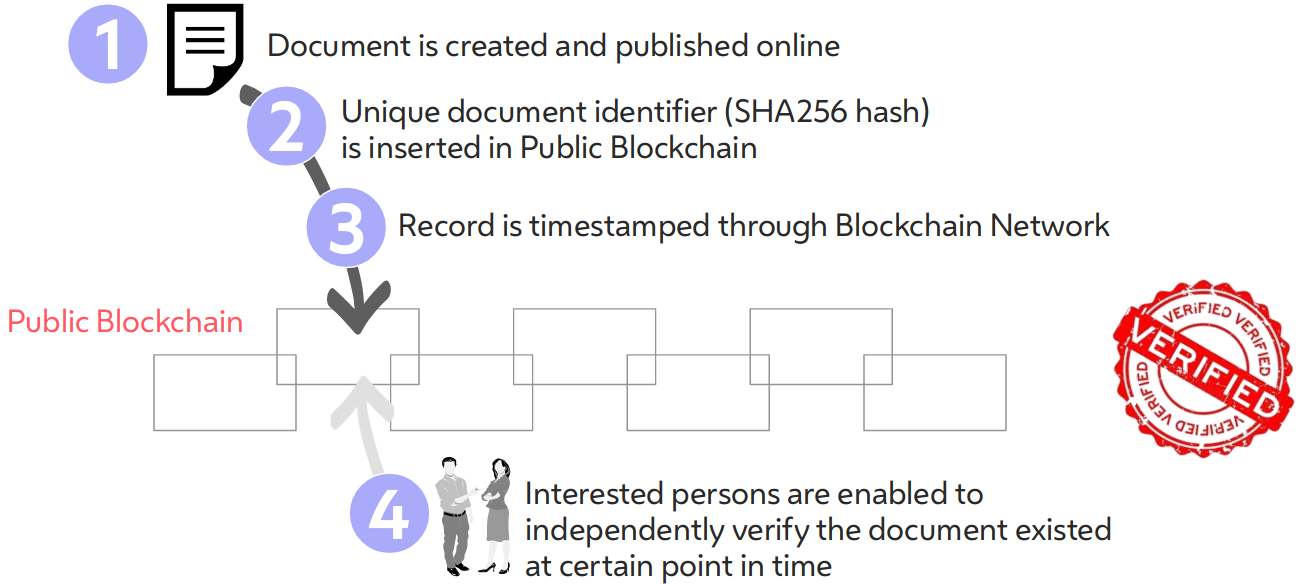
\includegraphics[width=.9\textwidth,height=.4\textwidth]{img/ViennaBc.png}
            % \caption{Vienna Blockchain notarization solution.}
            % \label{fig:arOv}
        \end{figure}}
\end{frame}

\section{Proposed Architecture}
\begin{frame}{Overview}{Architecture}
    Our system includes: \pause a \textbf{Portal}, \pause a distributed file storage system \textbf{IPFS} \pause and a private blockchain network \textbf{Hyperledger Fabric}.
    \pause
    \begin{figure}
        \centering
        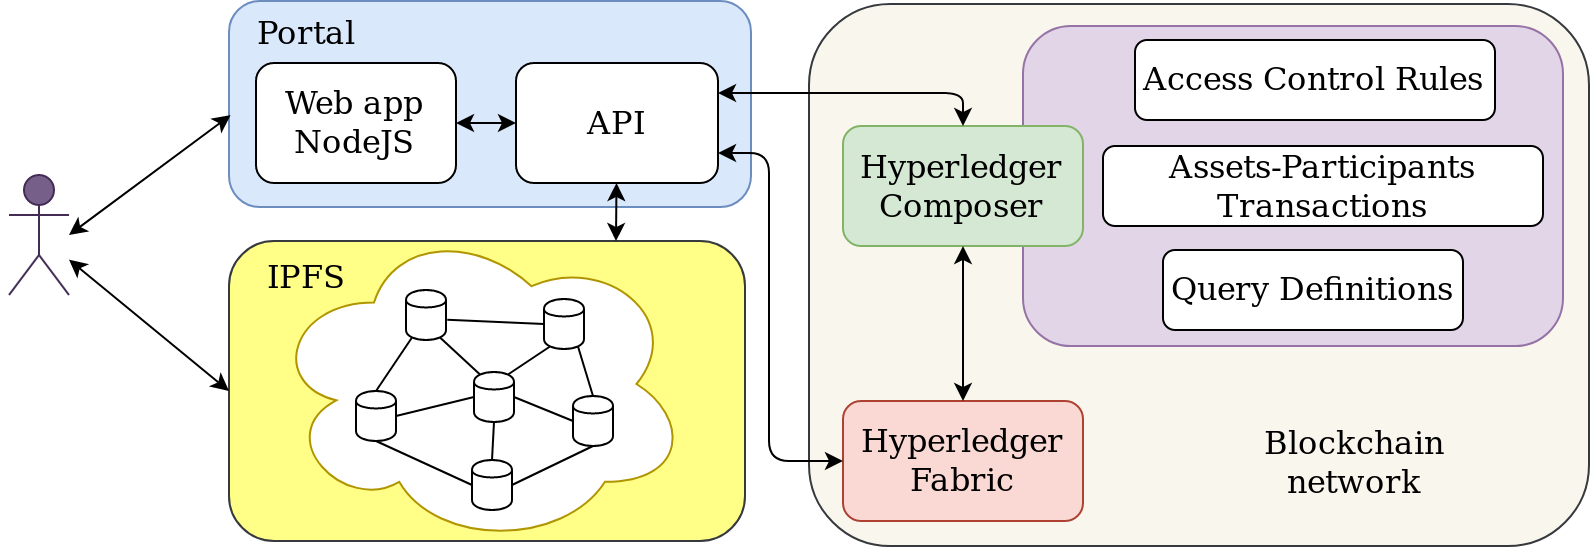
\includegraphics[width=.9\textwidth,height=0.4\textwidth]{img/ArOv.png}
        % \caption{Architecture overview}
        % \label{fig:arOv}
    \end{figure}
\end{frame}

\begin{frame}{Overview}{Explaining}
    Why Hyperledger Fabric and IPFS?
    \setbeamercovered{transparent}
    \begin{itemize}
        \uncover<2->{\item We want to decentralize our system as much as we can.}
              \uncover<3->{\item Hyperledger Fabric: authenticates data contributor, traces data log, checks data integrity, enhances the system transparency.}
              \uncover<4->{\item IPFS: ensures the data integrity and availability.}
    \end{itemize}
\end{frame}



% \begin{frame}{Overview}{Modules role}
%     \setbeamercovered{transparent}
%     \begin{itemize}
%         \onslide<1->{
%         \item[1.] The \textbf{Portal} \textit{handles user requests}:
%               % is responsible for interacting with two remaining parts.
%               \begin{itemize}
%                   %   \uncover<2->{
%                   %   \item<2-> handles user requests;
%                   %   }
%                   % \uncover<3->{
%                   \item<2-> Triggering smart contracts.
%                         % }
%                         % \uncover<4->{
%                   \item<3-> Uploading data to the IPFS.
%                         % }
%               \end{itemize}
%               }
%               \pause
%               \pause
%               \pause
%               %   \pause
%               \onslide<4->{
%         \item[2.] The \textbf{IPFS} \textit{enhances the data integrity and availability}:
%               \begin{itemize}
%                   \uncover<5->{
%                   \item Storing the data sets.
%                         }
%                         \uncover<6->{\item Generating the content-based address.}
%                         % \uncover<8->{\item enhances the data integrity and availability.}
%               \end{itemize}
%               }
%               %     \end{itemize}
%               % \end{frame}

%               % \begin{frame}{ Overview}
%               %     \setbeamercovered{transparent}
%               %     \begin{itemize}
%               \pause
%               \pause
%               \pause
%               %   \pause
%               \onslide<7->{
%         \item[3.] The \textbf{Hyperledger Fabric} \textit{improves system transparency, enhances integrity and manages system}:
%               % plays an important role in ensuring transparency and enhancing the data integrity.
%               \begin{itemize}
%                   \uncover<8->{\item Storing the metadata of the data sets.}
%                         \uncover<9->{\item Authenticating data contributors.}
%                         % \uncover<12->{\item enhances the system transparency;}
%                         \uncover<10->{
%                         % \item Providing a mechanism to distributed verify all data content.
%                   \item Distributed verifying data content.
%                         }
%               \end{itemize}
%               }
%     \end{itemize}
% \end{frame}

% \begin{frame}{ Hyperledger Fabric network}
%     The general structure of Hyperledger Fabric network:
%     \begin{figure}
%         \centering
%         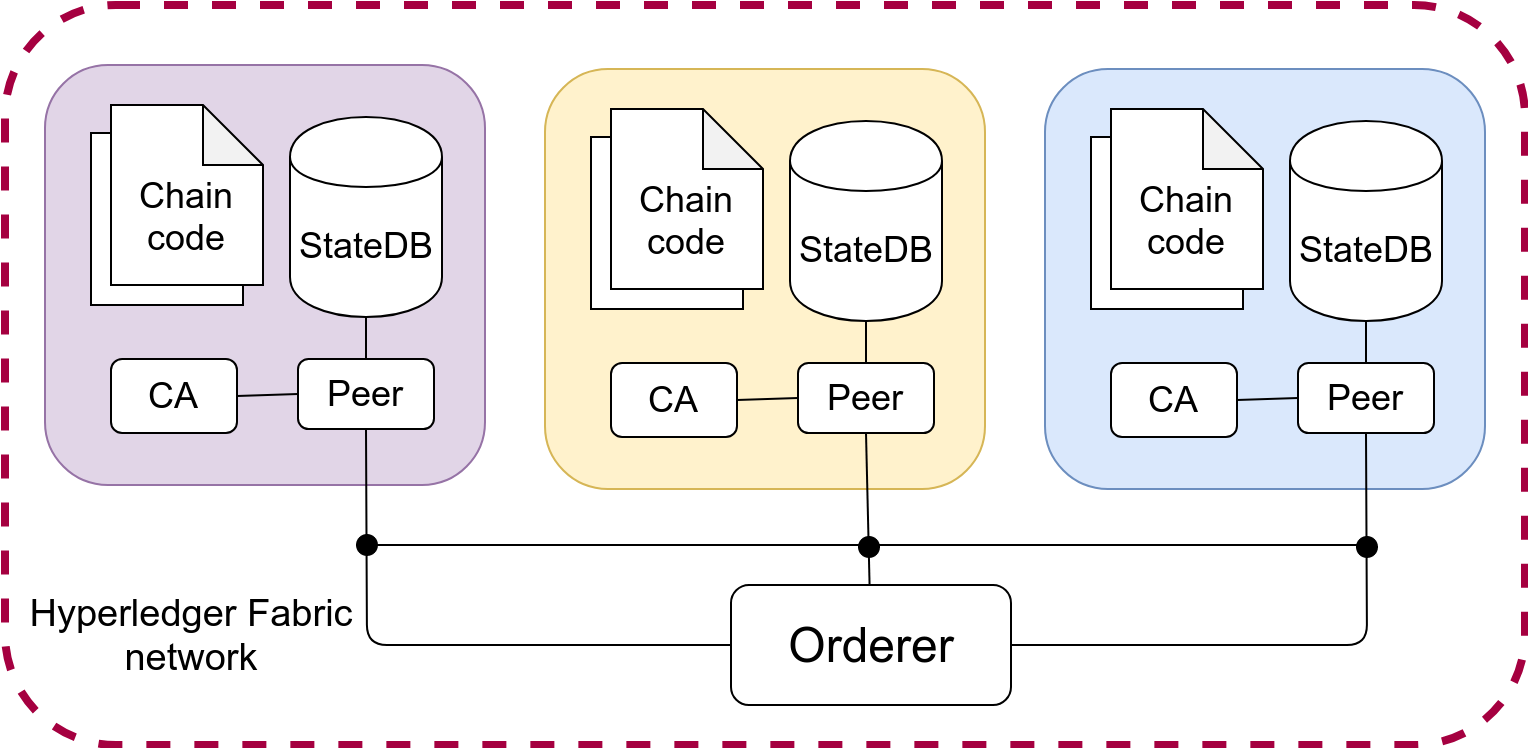
\includegraphics[width=.8\textwidth]{img/HFnet.png}
%         % \caption{Architecture overview}
%         % \label{fig:netArchi}
%     \end{figure}
% \end{frame}

% \begin{frame}{ Hyperledger Fabric network}
%     In the structure of the network, \textbf{organization}s represent ministries that contribute data to the open data portal.
%     \setbeamercovered{transparent}
%     \begin{itemize}
%         \uncover<2->{\item \textbf{Peers} participates in network operation.}
%               \uncover<3->{\item \textbf{Certificate Authority} issues and authenticates digital certificates.}
%               \uncover<4->{\item \textbf{Local database} includes \textit{world state} and \textit{blockchain ledger}.}
%               \uncover<5->{\item \textbf{Chaincode}.}
%     \end{itemize}
% \end{frame}


% \begin{frame}{ Hyperledger Fabric network}
%     \setbeamercovered{transparent}
%     \begin{itemize}
%         \onslide<1->{\item[+] \textbf{Chaincode}
%               \begin{itemize}
%                   \uncover<2->{\item handles business logic;}
%                         \uncover<3->{\item defines types of transactions, access control rules, type of participants, type of assets and custom queries;}
%                         \uncover<4->{\item triggers transactions to store metadata, user identity, and log events into the blockchain ledger and the distributed databases.}
%               \end{itemize}
%               }
%               \pause
%               \pause
%               \pause
%               \pause
%               \onslide<5->{\item[+] \textbf{Endorsement Policy} defines the number of node participating in the consensus process.}
%     \end{itemize}
% \end{frame}


\begin{frame}{System features}
    Our system has two main features:
    \begin{itemize}
        \item Publishing the data sets.
        \item Downloading-Verifying the data sets.
    \end{itemize}
\end{frame}

\begin{frame}{System features}{Publishing the data sets}
    \begin{center}
        \begin{figure}[H]
            \resizebox{0.8\linewidth}{!}{
                \begin{sequencediagram}
                    \renewcommand\unitfactor{0.5}
                    \newthread{B}{\textsf{Data Publisher}}{}
                    \newinst[1]{D}{\textsf{Server}}
                    \newinst[1]{F}{\textsf{IPFS}}
                    \newinst[1]{E}{\textsf{Hyperledger Fabric network}}
                    \begin{call}{B}{\textsf{Verify()}}{D}{result}
                    \end{call}
                    \begin{sdblock}{\textsf{alt}}{result=token}

                        \begin{call}{B}{\textsf{pubFunc()}}{D}{\textsf{return}}
                            \begin{call}{D}{\textsf{Authen()}}{E}{\textsf{result}}
                            \end{call}
                            \begin{sdblock}{alt}{result=true}
                                \begin{call}{D}{\textsf{upload()}}{F}{\textsf{data address}}
                                \end{call}
                                \begin{call}{D}{\textsf{pubTransac()}}{E}{\textsf{return}}
                                \end{call}
                            \end{sdblock}
                        \end{call}
                    \end{sdblock}
                \end{sequencediagram}}
            % \caption{The publishing data sets process.}
            % \label{fig:publishDataset}
        \end{figure}
    \end{center}
\end{frame}


\begin{frame}{System features}{Downloading-verifying the data sets}
    \begin{center}
        \begin{figure}[H]
            \resizebox{0.7\linewidth}{!}{
                \begin{sequencediagram}
                    \newthread{A}{\textsf{Citizens}}
                    \newinst[1]{D}{\textsf{Server}}
                    \newinst[1]{C}{\textsf{IPFS}}
                    \newinst[1]{E}{\textsf{Hyperledger Fabric network}}
                    \begin{call}{A}{\textsf{access()}}{D}{\textsf{return}}
                        \begin{call}{D}{\textsf{queryAllDatasets()}}{E}{\textsf{return}}
                        \end{call}
                    \end{call}
                    \begin{call}{A}{\textsf{downFunc()}}{D}{\textsf{return address}}
                        \begin{sdblock}{opt}{check data integrity}
                            \begin{call}{A}{\textsf{isDataValid()}}{D}{\textsf{return}}
                                \begin{call}{D}{\textsf{download()}}{C}{\textsf{return}}
                                \end{call}
                                \begin{call}{D}{\textsf{VerifyData()}}{E}{\textsf{return}}
                                \end{call}
                            \end{call}
                        \end{sdblock}
                    \end{call}
                    \begin{call}{A}{\textsf{download()}}{C}{\textsf{return}}
                    \end{call}
                \end{sequencediagram}}
            % \caption{The downloading-verifying process.}
            % \label{fig:downloadData}
        \end{figure}
    \end{center}
\end{frame}

\section{Implementation}
\begin{frame}{Implementation}

    Our implementation included:
    \begin{itemize}
        \item Hyperledger Fabric network
        \item The open data portal
    \end{itemize}
\end{frame}

% \begin{frame}{Hyperledger Fabric network}{Building network}
%     We construct our blockchain network according to Hyperledger project guideline\footnote{Blockchain Development with Hyperledger: Build decentralized applications with Hyperledger Fabric and Composer, 2019}.
%     \setbeamercovered{transparent}
%     \begin{itemize}
%         \uncover<2->{\item Set up environment: peers, orderer, couchDB databases, CA.}
%               \uncover<3->{\item Connect modules together.}
%               \uncover<4->{\item Define customize chaincode: paticipants, assets, transactions, access control, endorsement policy.}
%     \end{itemize}
% \end{frame}

\begin{frame}{Hyperledger Fabric network}{Hyperledger Composer}
    % \begin{block}{Hyperledger Composer}
    \textbf{Hyperledger Composer} is an extensive, open development toolset and framework to make developing blockchain applications easier.
    % \end{block}
    \pause
    \begin{figure}
        \centering
        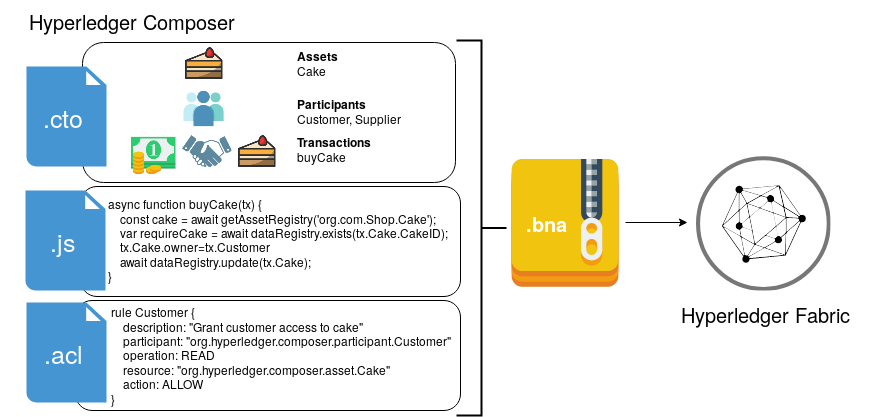
\includegraphics[width=\textwidth,height=0.45\textwidth]{img/HC.png}
        % \caption{Architecture overview}
        % \label{fig:arOv}
    \end{figure}
\end{frame}

\begin{frame}{Hyperledger Fabric network}{Chaincode}
    We use Hyperledger Composer to define our customize chaincode.
    \setbeamercovered{transparent}
    \begin{itemize}
        \onslide<1->{\item[1.]Participants, Assets
              \begin{itemize}
                  \uncover<2->{\item The data contributors represented as \textbf{DataPublisher} object.}
                        \pause
                        \pause
                        \onslide<3->{\lstinputlisting[language=modelLang]{code/Publisher.txt}}
                        \uncover<4->{\item The metadata of the data sets represented as \textbf{Data} object.}
                        \pause
                        \pause
                        \onslide<5->{\lstinputlisting[language=modelLang]{code/Data.txt}}
              \end{itemize}
              }
    \end{itemize}
\end{frame}
\begin{frame}{Hyperledger Fabric network}{Chaincode}
    \setbeamercovered{transparent}
    \begin{itemize}
        \onslide<1->{\item[2.]Transactions
              \begin{itemize}
                  \uncover<2->{\item Publish the data sets process: \textbf{AddAsset()}, \textbf{PublishData()}}
                        \pause
                        \pause
                        \onslide<3->{\lstinputlisting[language=modelLang]{code/PublishData.txt}}
                        \uncover<4->{\item Modify and Verify the data sets process: \textbf{ModifyData()} \textbf{VerifyData()}}
                        \pause
                        \pause
                        \onslide<5->{\lstinputlisting[language=modelLang]{code/ModifyData.txt}}
              \end{itemize}
              }
    \end{itemize}
\end{frame}
\begin{frame}{Hyperledger Fabric network}{Chaincode}
    \setbeamercovered{transparent}
    \begin{itemize}
        \onslide<1->{\item[3.]Access control
              \begin{itemize}
                  \uncover<2->{\item The data contributor permission.}
                        \uncover<3->{\item The citizens permission.}
                        \pause
                        \pause
                        \pause
                        \onslide<4->{\lstinputlisting[language=modelLang]{code/ACL.txt}}
              \end{itemize}
              }
    \end{itemize}
\end{frame}
\begin{frame}{Hyperledger Fabric network}{Endorsement Policy}
    \begin{itemize}
        \item[4.]Endorsement Policy
              \lstinputlisting[language=modelLang]{code/EP.txt}
    \end{itemize}
\end{frame}
\begin{frame}{Open data portal}
    \setbeamercovered{transparent}
    \onslide<1->{
        \textbf{Server-side} implementation:
        \begin{itemize}
            \uncover<2->{\item Written by NodeJS.}
                  \uncover<3->{\item Using Hyperledger Composer to interact with Hyperledger Fabric blockchain network.}
                  \uncover<4->{\item Connecting to IPFS network.}
        \end{itemize}}
    \pause
    \pause
    \pause
    \pause
    \onslide<5->{
        \textbf{Client-side} implementation:
        \begin{itemize}
            \uncover<6->{\item  Written by VueJS.}
        \end{itemize}}
\end{frame}

\section{Testing}
\begin{frame}{Testing}
    \onslide<1->{\textbf{Hyperledger Caliper}\footnote{\url{https://github.com/hyperledger.caliper}} is a blockchain performance benchmark framework.}
    % which allows users to test different blockchain solutions with predefined use cases, and get a set of performance test results.}
    \pause
    \onslide<2->{
        \begin{table}[H]
            \centering
            \captionsetup{justification=centering}
            \captionof{table}{Evaluated result of blockchain network performance\\Number of transactions: 100, transactions rate: 100 tps}
            \label{tab:result}
            \resizebox{\columnwidth}{!}{%
                \begin{tabular}{@{}cccccc@{}}
                    \toprule
                    \multirow{2}{*}{\textbf{Transaction type}} & \multirow{2}{*}{\textbf{\begin{tabular}[c]{@{}c@{}}Send rate\\ (tps)\end{tabular}}} & \multicolumn{3}{c}{\textbf{Latency (s)}} & \multirow{2}{*}{\textbf{\begin{tabular}[c]{@{}c@{}}Throughput\\ (tps)\end{tabular}}}                                          \\ \cmidrule(lr){3-5}
                                                               &                                                     & \multicolumn{1}{l}{\textbf{Min}}         & \multicolumn{1}{l}{\textbf{Max}}                    & \multicolumn{1}{l}{\textbf{Avg}} &     \\ \midrule
                    PublishData                                & 96.4                                                & 6.45                                     & 16.08                                               & 11.73                            & 6.1 \\
                    ModifyData                                 & 101.0                                               & 6.60                                     & 15.67                                               & 11.27                            & 6.3 \\
                    DownloadData                               & 100.6                                               & 6.66                                     & 16.09                                               & 11.06                            & 6.1 \\ \bottomrule
                \end{tabular}
            }
        \end{table}}
\end{frame}

\section{Conclusion}
\begin{frame}{Conclusions}
    \setbeamercovered{transparent}
    \begin{itemize}
        \onslide<1->{\item[+] The combination of the Hyperledger Fabric and the IPFS technology enhances the transparency, availability and integrity of the open data.}
              \medskip
              \pause
              \onslide<2->{\item[+] The limitation:
              \begin{itemize}
                  \uncover<3->{\item storing the private key of the publisher.}

              \end{itemize}}
              \medskip
              \pause
              \pause
              \onslide<4->{\item[+] Future works:
              \begin{itemize}
                  \uncover<5->{\item integrating hardware security modules;}
                        \uncover<6->{\item evaluatating the performance of the IPFS network.}
              \end{itemize}}
    \end{itemize}

\end{frame}



\begin{frame}{Q\&A}
    \begin{figure}
        \centering
        
\includegraphics[width=0.8\textwidth,height=0.4\textwidth]{img/Q-A.png}
        % \caption{Architecture overview}
        % \label{fig:arOv}
    \end{figure}
\end{frame}
%------------------------------------------------


%------------------------------------------------
%------------------------------------------------

% \begin{frame}
% \titlepage 
% \end{frame}


\end{document}